\documentclass{sigchi}

% Use this command to override the default ACM copyright statement (e.g. for preprints). 
% Consult the conference website for the camera-ready copyright statement.


%% EXAMPLE BEGIN -- HOW TO OVERRIDE THE DEFAULT COPYRIGHT STRIP -- (July 22, 2013 - Paul Baumann)
% \toappear{Permission to make digital or hard copies of all or part of this work for personal or classroom use is 	granted without fee provided that copies are not made or distributed for profit or commercial advantage and that copies bear this notice and the full citation on the first page. Copyrights for components of this work owned by others than ACM must be honored. Abstracting with credit is permitted. To copy otherwise, or republish, to post on servers or to redistribute to lists, requires prior specific permission and/or a fee. Request permissions from permissions@acm.org. \\
% {\emph{CHI'14}}, April 26--May 1, 2014, Toronto, Canada. \\
% Copyright \copyright~2014 ACM ISBN/14/04...\$15.00. \\
% DOI string from ACM form confirmation}
%% EXAMPLE END -- HOW TO OVERRIDE THE DEFAULT COPYRIGHT STRIP -- (July 22, 2013 - Paul Baumann)


% Arabic page numbers for submission. 
% Remove this line to eliminate page numbers for the camera ready copy
\pagenumbering{arabic}


% Load basic packages
\usepackage{balance} % to better equalize the last page
\usepackage{graphics} % for EPS, load graphicx instead
\usepackage{times}  % comment if you want LaTeX's default font
\usepackage{url}   % llt: nicely formatted URLs
\usepackage{listings}
\usepackage{color}
\usepackage[english]{babel}
\usepackage{setspace}

\definecolor{mygreen}{rgb}{0,0.6,0}
\definecolor{mygray}{rgb}{0.5,0.5,0.5}
\definecolor{mymauve}{rgb}{0.58,0,0.82}
\definecolor{black}{rgb}{0,0,0}

\lstset{ %
  backgroundcolor=\color{white},   % choose the background color; you must add \usepackage{color} or \usepackage{xcolor}
  basicstyle=\scriptsize\ttfamily,        % the size of the fonts that are used for the code
  breakatwhitespace=false,         % sets if automatic breaks should only happen at whitespace
  breaklines=true,                 % sets automatic line breaking
  captionpos=b,                    % sets the caption-position to bottom
  commentstyle=\color{mygreen},    % comment style
  deletekeywords={...},            % if you want to delete keywords from the given language
  escapeinside={\%*}{*)},          % if you want to add LaTeX within your code
  extendedchars=true,              % lets you use non-ASCII characters; for 8-bits encodings only, does not work with UTF-8
  frame=single,                    % adds a frame around the code
  keepspaces=true,                 % keeps spaces in text, useful for keeping indentation of code (possibly needs columns=flexible)
  keywordstyle=\color{blue},       % keyword style
  %language=Octave,                 % the language of the code
  morekeywords={*,...},            % if you want to add more keywords to the set
  numbers=left,                    % where to put the line-numbers; possible values are (none, left, right)
  numbersep=5pt,                   % how far the line-numbers are from the code
  numberstyle=\tiny\color{mygray}, % the style that is used for the line-numbers
  rulecolor=\color{black},         % if not set, the frame-color may be changed on line-breaks within not-black text (e.g. comments (green here))
  showspaces=false,                % show spaces everywhere adding particular underscores; it overrides 'showstringspaces'
  showstringspaces=false,          % underline spaces within strings only
  showtabs=false,                  % show tabs within strings adding particular underscores
  stepnumber=2,                    % the step between two line-numbers. If it's 1, each line will be numbered
  stringstyle=\color{black},     % string literal style
  tabsize=2,                       % sets default tabsize to 2 spaces
  title=\lstname                   % show the filename of files included with \lstinputlisting; also try caption instead of title
}

% llt: Define a global style for URLs, rather that the default one
\makeatletter
\def\url@leostyle{%
 \@ifundefined{selectfont}{\def\UrlFont{\sf}}{\def\UrlFont{\small\bf\ttfamily}}}
\makeatother
\urlstyle{leo}


% To make various LaTeX processors do the right thing with page size.
\def\pprw{8.5in}
\def\pprh{11in}
\special{papersize=\pprw,\pprh}
\setlength{\paperwidth}{\pprw}
\setlength{\paperheight}{\pprh}
\setlength{\pdfpagewidth}{\pprw}
\setlength{\pdfpageheight}{\pprh}

% Make sure hyperref comes last of your loaded packages, 
% to give it a fighting chance of not being over-written, 
% since its job is to redefine many LaTeX commands.
\usepackage[pdftex]{hyperref}
\hypersetup{
pdftitle={SIGCHI Conference Proceedings Format},
pdfauthor={LaTeX},
pdfkeywords={SIGCHI, proceedings, archival format},
bookmarksnumbered,
pdfstartview={FitH},
colorlinks,
citecolor=black,
filecolor=black,
linkcolor=black,
urlcolor=black,
breaklinks=true,
}

% create a shortcut to typeset table headings
\newcommand\tabhead[1]{\small\textbf{#1}}


% End of preamble. Here it comes the document.
\begin{document}

\title{DressCode: Subtitle to come}

\numberofauthors{3}
\author{
 \alignauthor 1st Author Name\\
  \affaddr{Affiliation}\\
  \affaddr{Address}\\
  \email{e-mail address}\\
  \affaddr{Optional phone number}
 \alignauthor 2nd Author Name\\
  \affaddr{Affiliation}\\
  \affaddr{Address}\\
  \email{e-mail address}\\
  \affaddr{Optional phone number}
}

\maketitle

\begin{abstract}
\end{abstract}

\keywords{
	Guides; instructions; author's kit; conference publications;
	keywords should be separated by a semi-colon.
}

\category{H.5.m.}{Information Interfaces and Presentation (e.g. HCI)}{Miscellaneous}

\section{Introduction} %clean up to emphasize priorities #1 accessible computational design tools for young people, #2 relevant contexutalization of tools through activity design incorporating craft
There is a growing emphasis on teaching young people skills in technological production to advance our societal technological progress. A common component of these learning initiatives is that they seek to provide students with skills for \textit{future} careers in technology. We believe in the value of working with young people in technological production, but draw upon Dewey's observation that education oriented towards future responsibilities can hinder active participation by students in the present \cite{dewey}. Furthermore, we recognize that limited participation in STEM fields by women and minorities is partly due to the perception that STEM applications themselves are constrained in cultural and intellectual diversity and breadth \cite{buechley_wild}. To successfully engage a diverse population of young people in technology-based creation requires two components. First we must develop tools that are accessible and appealing to then.  Second, we must apply these tools to forms of creation that are relevant to their \emph{current} lives and personal interests. Computational design provides an opportune space to achieve these objectives. Prior research has demonstrated that physical craft practices offer a compelling way to engage young people in computation. Building off of this work, we explored the application of novice-accessible computational design for craft through the creation of a stand-alone computational design software aimed at young novice programmers, and a activity design employing this tool in the production of wearable artifacts.

The process of combining craft and computational design raises several important questions. Foremost, what are important design principles to consider when developing computational design tools for young people? What methods are helpful in ensuring accessibility, creative flexibility, and support of computational affordances? Furthermore, how can both the software and the activity structure reduce technical and conceptual challenges in translating a computational design into a viable physical artifact? Lastly, what values are reflected in this form of production, what range of young people are engaged by this form of making, and how are the resulting artifacts applicable to their lives?

To explore these questions we have developed our own computational software, DressCode, which features linked editable representations between programing code and graphic drawing and manipulation. In the process of developing DressCode, we prototyped several specific craft activities in sewing, jewelery making and t-shirt design. We used this process as the basis for the development of an activity design which we evaluated in one preliminary and one long term workshop with high-school students where participants designed and produced jewelery and printed onto clothing. In this paper, we detail the features of the DressCode software, the principles of our computational activity design for young people, and our methodology and results from the workshops. Through analysis of these experiences, we describe design factors that enable young people to computation and making in ways that emphasize pleasure, exploration, intellectual engagement and utility in the service of personal expression. We conclude with a set of recommendations for the development of tools and activities for future forms of engagement in computational design and making.

\section{Creative Opportunities in Computational Design}
Papert and collaborators recognized early on that computer programing can serve as a way for children to learn powerful ideas about mathematics, geometry and logic \cite{mindstorms}. In computational design, programming provides a powerful way of thinking about design in direct relation to math and logic. Additionally, computational design offers a unique approach to the design process itself. Computational design is best represented as a way of applying procedural thinking to a design task. Designers author rules that define systems capable of producing many outcomes, enabling the production of  multiple design variations that share a set of constraints. Through this systematic abstraction, the following are possible \cite{reas}:
\begin{itemize}
\item \textbf{Precision:} Computation supports high levels of numerical precision.
\vspace{-8pt}
\item \textbf{Visual Complexity:} Computational design allows for rapid creation and transformation of complex patterns and structures, allowing for complex manipulations of numerous design elements.
\vspace{-6pt}
\item \textbf{Generativity:} Designers create algorithms that allow for the computer to autonomously produce unique and unexpected designs.
\vspace{-6pt}
\item \textbf{Parameterization:} Computation allows users to specify a set of degrees of freedom and constraints of a model and then adjust the values of the degrees of freedom while maintaining the constraints.
\vspace{-6pt}
\item \textbf{Remixing:} Computationally generated designs are created by a program which can be modified by other designers. 
\end{itemize} 
%Computational design also contains a number of unique challenges: bring these up in discussion
%\begin{itemize}
%\item \textbf{Formalizing complex problems} As design problems grow in complexity, formalizing the problem in a manner that can be expressed programmatically becomes challenging. 
%\item \textbf{Creating singularities:} A designer will often choose to deviate from a set pattern or structure at specific points in order to create a special emphasis in the area of deviation. Because computational design is governed by a systematized ruleset, the methods of breaking these rules at arbitrary points are often unclear or tedious to implement. 
%\item \textbf{Selecting a final design:} Computational design gives the designer the ability to produce extremely large numbers of solutions to a single design problem. While this is useful in situations where multiple solutions are required, when a single design must be chosen, the process of deciding on a solution is difficult, especially if the decision is based on aesthetic criteria.
%\end{itemize}
\subsection{Challenges in Access and Application}
Although amatuer use of computational design growing, it remains largely inaccessible to individuals who are new to programing. This is in part due to practical and technical barriers. Many of the programming languages used for computational design are difficult for novices to learn and most novice oriented programming environments emphasize producing screen-based work rather than physical objects. Novice-oriented computer-aided-design (CAD) software emphasizes graphic interaction and seldom features computational methods as a key design tool. Significant perceptual barriers also exist. Many people consider programming to be irrelevant to their interests, and are unmotivated to pursue what they perceive to be a highly specialized and difficult undertaking \cite{resnick1}. There also are perceptions of technology in general which may engagement by people who are interested in making. Digital technology is often portrayed as reducing the need or desire for manual human labor, rather than supporting it in creative forms \cite{rosner_craft_vs_design}.

\section{Related Work}
We examined several fields of related software tools including learning-oriented programing environments, Computer Aided Design (CAD) tools with computational functionality, as well as digital design tools with linked forms of editing. We also considered prior research in combining craft, computational design for young people.

\subsection{Learning Oriented Programing Environments}
Logo is the seminal novice programming language founded on principles of constructionism and embodiment \cite{papert}. The Scratch programing environment was developed as a successor to Logo. Scratch is one of the most successful modern novice-oriented programming environments, and allows users to create interactive projects by combining command blocks \cite{resnick2}. Processing is a language and development environment for creating complex forms and animations. Described as an entry level programming environment, Processing has also become a successful professional computational design tool\cite{processing}. Although neither Logo, Scratch or Processing were explicitly created for compatibility with craft practices, they share features that enable creative programing by novices. They contain a simplified programming syntax, prioritize visual feedback, and are applicable to a diverse range of projects and interests.
%discuss codeable objects

\subsection{CAD tools with Computational Design Functionality} %make this about computational design tools for novices
Arguably, computational design can be performed with any programming language that has the capability to output some form of graphic data. A number of CAD tools have been developed that explicitly feature computational design through programing. Most are designed for professional users. In Adobe software like Photoshop and Illustrator, it is possible to write Javascript-based programs to automate various application procedures. Similarly, 3D modeling tools such as Maya and Blender feature the ability to script behaviors in languages that are syntactically similar to Perl and Python, respectively. In all of these examples the programming interface is omitted from the primary interfaces of the application and must be deliberately activated by the user. Other computational design and CAD tools feature a more direct emphasis on programing in their interface. Grasshopper is data-flow programming environment that enables users to combine a variety of visual modules and blocks to create and adjust 3D models in Rhino \cite{grasshopper}, and DesignScript, an add-on to the Autodesk AutoCad software  that allows users to computationally create 3D architectural forms through a combination of associative and imperative programing paradigms in an effort to support a pedagogical transition between basic and advanced levels of programming \cite{DesignScript}. OpenSCAD is a script-based constructive solid-geometry modeling tool developed specifically for CAD applications. OpenSCAD contains a custom programming language in which the user can create descriptions of 3D models in a textual format and display them by compiling the script\cite{OpenScad}.

Novice-oriented CAD tools with computational design features are rare, but some examples do exist. FlatCAD seeks to connect programming and digital fabrication, and allows users to build customized construction kits with a laser cutter by programming in FlatLang, a novice-oriented programming language modeled on Logo \cite{flatcad}. TinkerCad is 3D-modeling tool designed for entry level users to create forms for 3d printing. TinkerCAD recently added "shape scripts", functionality enabling the creation of javascript programs that produce 3D forms \cite{tinkercad}.

\subsection{Linked Editors}
Avrahami, Brooks and Brown demonstrated an early approach to a two-view system for designing user interfaces by combining a graphic editor with direct manipulation of interface elements with a special-purpose programming language. Interface designs can be edited in either view, and the changes are reflected in the other view \cite{two_view_ui}. Commercially, the two-view approach has been incorporated primarily into web editors \cite{dreamweaver}and UI design tools in software development kits \cite{eclipse}, \cite{something else}. Victor has convincingly advocated for the incorporation of a of forms of linked representations in a broad range of fields including circuit design, game development and graphic design. His approach has been to advocate through the development of demonstrative examples rather than functioning tools \cite{victor}. Educational researchers have also found multiple linked representations to be advantageous in supporting learning \cite{white}. When applied to the appropriate context, multiple external representations can reduce the amount of cognitive effort required to solve a problem, and often better communicate complex content \cite{ainsworth}.

\subsection{Craft and Computing Research}
Eisenberg and Buechley's research on pervasive fabrication provides a foundation for our objectives combining computational design and craft. Their research encompasses techniques and approaches for incorporating digital fabrication into educational settings, and describes how fabrication enables youth to decorate their environments, allows them to create novel artifacts in the service of personal expression, and stimulates intellectual development \cite{pervasive_fab}. 

The development of DressCode is a direct successor to the research by Jacobs and Buechley on combining computational design and fashion. Jacobs and Buechley created a Processing-based programing library entitled Codeable Objects, to facilitate a series of workshops where young people produced fashion accessories and clothing by creating designs computationally and realizing them through a combination of digital fabrication and manual sewing and crafting \cite{codeable_objects}. Although our work is motivated by the rich engagement opportunities illustrated by Codeable Objects research, we are primarily interested developing a stand-alone design tool for novice computational design that combines textual programing with graphic drawing and manipulation. By developing a tool with linked representations, we seek to address the issues Jacobs and Buechley describe in their use of Processing with novice coders; including difficulties learning programing syntax, a frustration with the lack of visual feedback, and the need for frequent instructor assistance in technical programing tasks. 


\section{Dress Code Software Description}
DressCode is a 2D computational design tool that is distinguished by its support of \emph{linked editable representations} of a design in two forms: programmatic and graphic. As designs create and manipulate forms graphically, the software generates readable, editable programming expressions that correspond to their actions. designs can also generate graphic forms by writing programming expressions and manipulate these forms with the graphic editing tools. Here, we describe the interface and toolset of DressCode, the interaction paradigm by which a design creates a design, and the technical implementation that facilitates this paradigm.

\begin{figure*}
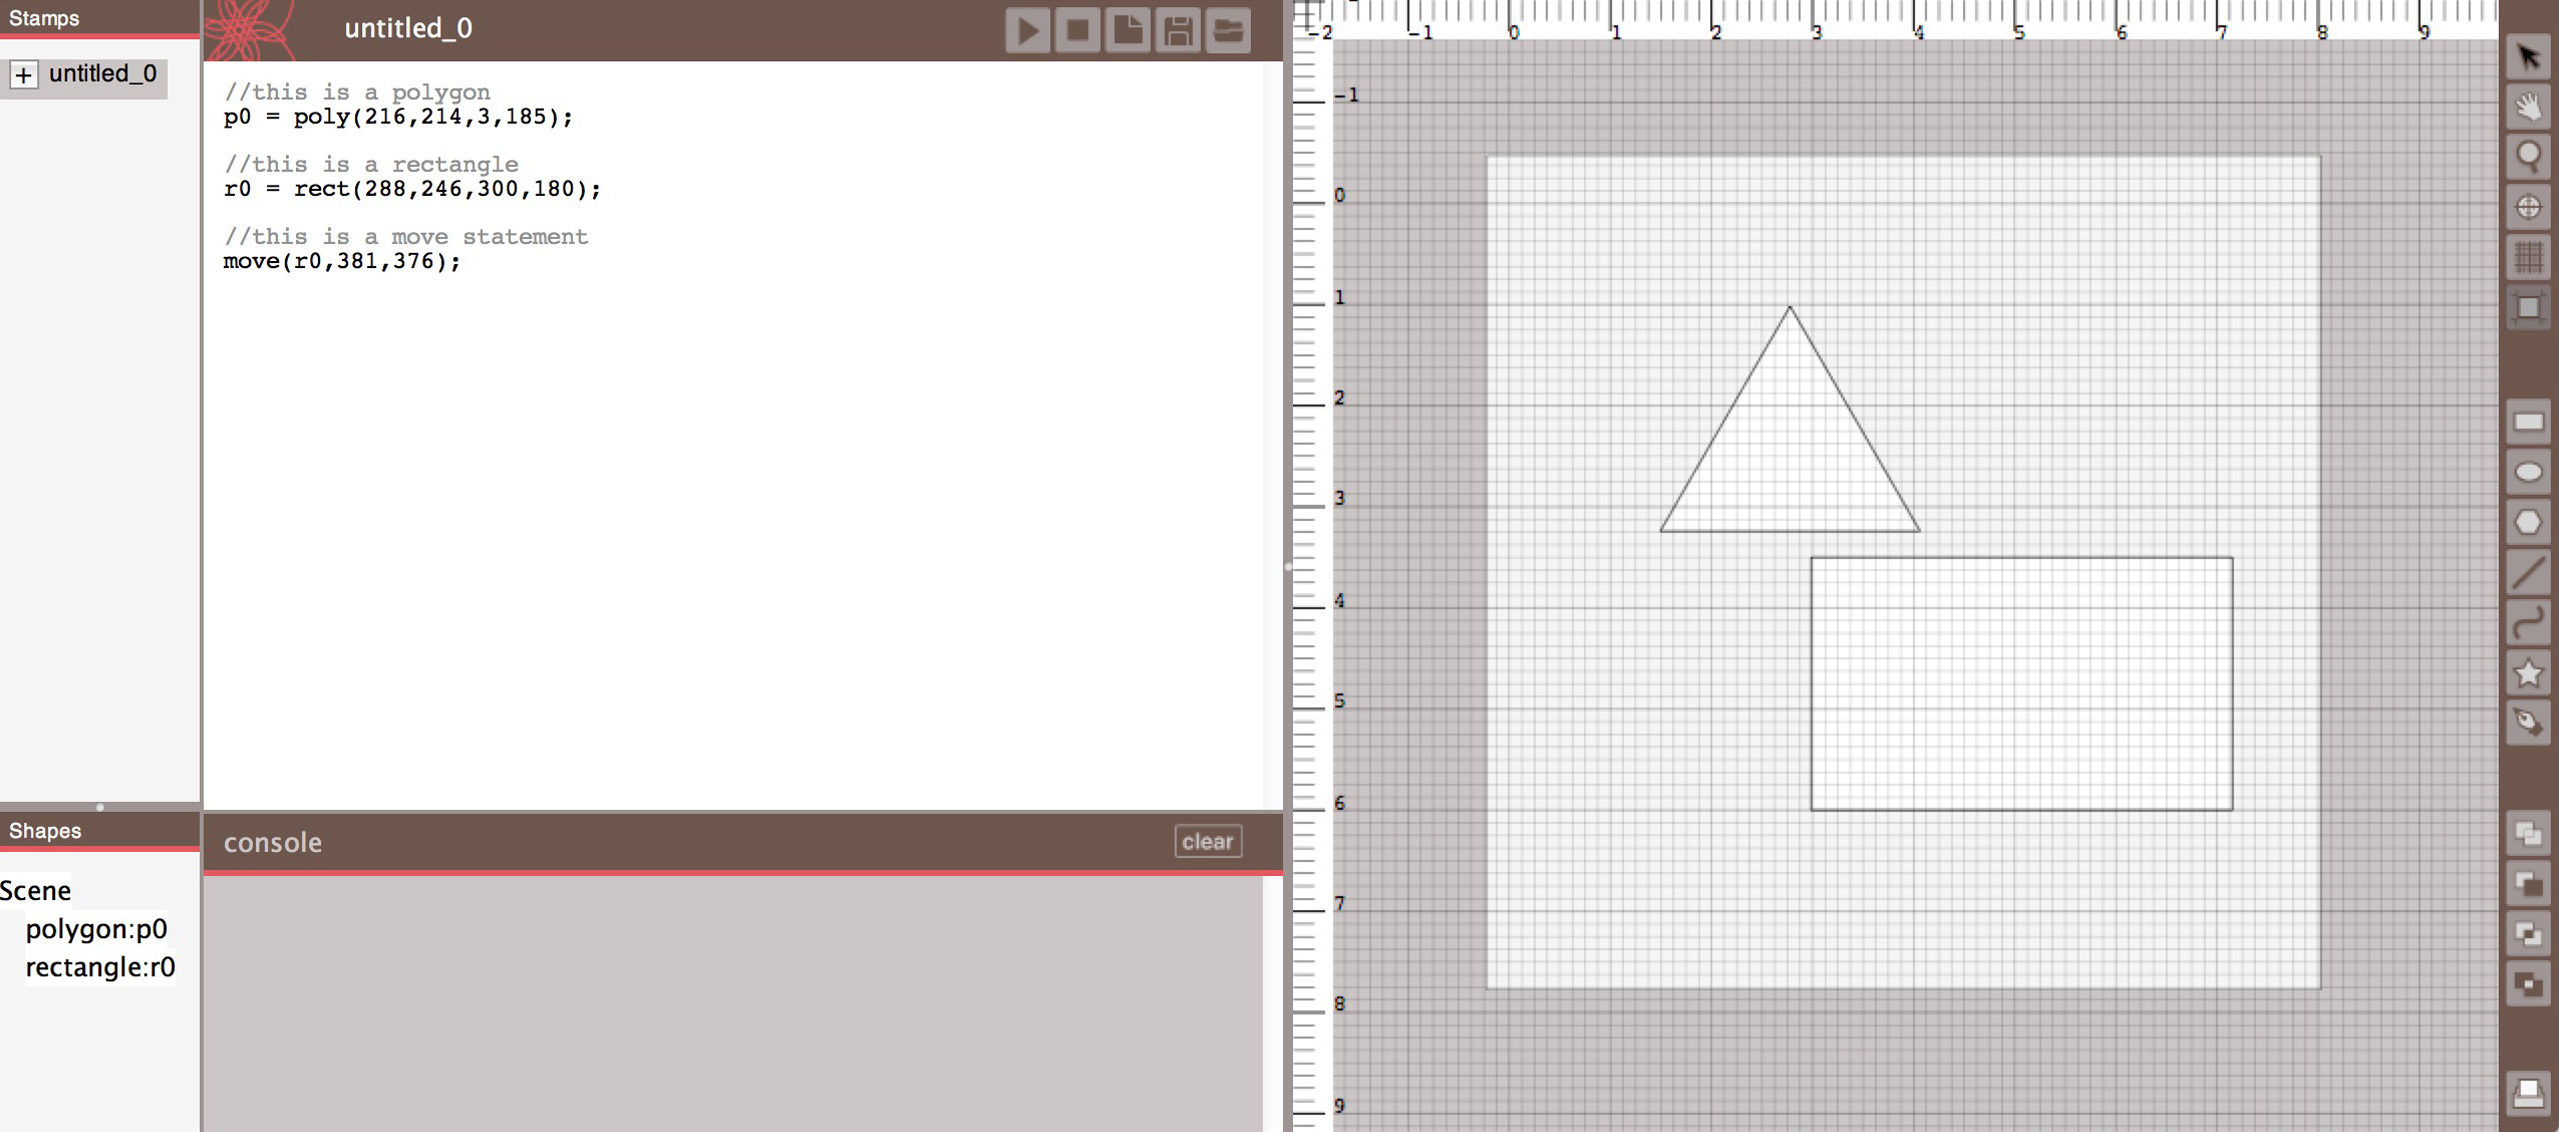
\includegraphics[width=\textwidth]{images/application_image_sm_content.jpg}
\caption{The DressCode Software)}
\label{fig:application_image}
\end{figure*}

\subsection{System Overiew}
The DressCode application resmbles a mashup of a digital graphic drawing tool, and a text editor. The interface iself it divided into two primary panels; a graphic panel on the right and a text editor panel on the left (figure:\ref{fig:application_image}). A design may write and execute programs using the text editor; similarly they can draw and manipulate shapes using the mouse in the graphic panel. Each panel contains specific features and tools to enable these respective interactions. The text editor contains a console for output and error messages, and a panel with buttons for compiling and running the current program, and terminating the compilation process. The design panel contains a re-sizable drawing board and grid with rulers corresponding to real-world units (inches and millimeters), and pan and zoom tools to facilitate navigation. A toolbar on the right-hand side of the graphic panel contains a menu of drawing and manipulation tools. It also contains a print tool which allows the design to export their current visual design in vector format for output through printing, or 2-axis forms of digital fabrication (figure:\ref{fig:graphic_tools}).

\begin{center}
\begin{figure}[h!]

\includegraphics[width=\columnwidth]{images/graphic_tools.jpg}
\caption{The graphic drawing and manipulation tools in DressCode (from left to right: selection and move tool, rectangle tool, ellipse tool, regular polygon tool, line tool, curve tool, SVG import tool, pen tool)}
\label{fig:graphic_tools}
\end{figure}
\end{center}
\vspace{-20pt}

The graphic drawing tools include regular primitive creation tools and a pen tool for the creation of irregular forms.  In addition to the drawing tools, the selection tool allows for individual primitives and groups to be manually selected and moved, and the boolean operation tools allow for the combination of two or more forms into a unified shape through a variety of polygon boolean operators (union, difference, intersection and either/or). The interface also contains two additional panels, the stamp panel and the declarative view which are described in the organizational structures subsection.

 DressCode contains a custom functional programing language which enables 2D drawing functionality via text expressions. The language supports conventional programming data-types, as well as loops, conditional expressions and design-defined functions. Variables in DressCode are dynamically typed and identifiers can be assigned to data-types that differ from their original assignment. The DressCode language contains a subset of expressions which facilitate the drawing and transformation of 2D graphic geometric forms. Lastly, the language supports basic math expressions and enables a variety of random noise generation methods. We discuss the drawing elements of the DressCode programing language and their relationship with the graphic manipulation tools at length in the following section. A note on terminology: for the remainder of this paper, we denote actions made in the graphic panel with the mouse as \textit{graphic actions}, and actions made in the programing panel by typing expressions as \textit{programatic actions}.


\subsection{Linked Representations In Practice}
Graphic tools and programing tools each have their own design affordances. Graphic tools are based on the metaphor of drawing and manipulation with traditional media, and often represented by icons and symbols reflecting this metaphor. As a result, they can be intuitive or inviting to new designs. Textual programing tools are often less intuitive, but have the advantage of readily supporting complexity and automation in design, and are a natural fit for parametric representations. Because of their differences, combining computational and graphic design into a unified interaction raises many questions and opportunities for different forms of interaction: What forms of interaction best support the distinct affordances of graphic manipulation and programing? How should graphical organizational structures be reconciled with computational forms of organization? What rules dictate the resolution of inevitable conflicts between graphical and programmatic actions? How does the intended application of the software dictate the relationships between the two paradigms?

In respect to these questions, we describe the DressCode's interaction structure, which we have based on primary design principles: Symmetry and Readability. In this section, we describe the latest state of the tool, which was iteratively developed through a series of workshops. The workshops not only directed the iterations of the tool itself, but assisted in the clarification of the design principles behind it. We discuss this development process at length in the workshop section. For now, we will describe the specific structures of the current version of DressCode as they correspond to symmetry and readability.

\subsection{Symmetry}
The governing design principle in DressCode is symmetry between programmatic actions and graphic actions. For every drawing-oriented programmatic action in a designs' program, a graphic element is generated or manipulated in the graphic view. Conversely, for each graphic action, a corresponding programing expression (or set of expressions) will appear in the text editor, within the lines of the designer's program. The DressCode programing language syntax was developed expressly to support this translation. 

\subsubsection{Auto-generated programing expressions}
The drawing API is formulated on an Object Oriented Programming paradigm where basic shapes (points, lines, curves, polygons etc.) are initialized by calling the appropriate method and passing it a set of parameters designating it's location and dimensions. If a shape is generated graphically, it's parameters are determined by the mouse gestures of the designer (where they click to determine the origin, and how far they drag from the origin to determine the dimensions). A new programing expression appears in the designer's program with its method determined by the type of graphic tool that was used to create the shape, and the parameters determined by the graphically defined dimensions. (points, lines, curves, polygons etc.) Shapes are layered in a design in order of the designer's graphic and programmatic actions, with shapes that were drawn most recently appearing on top of those created earlier.

Transformation methods, including moving, scaling, rotation, color and stroke changes, and shape booleans follow a similar structure to shape initialization. In the DressCode programing language, transformations are performed by either wrapping a shape-initialization expression in an a transformation expression, or by assigning an identifier to the shape, and then calling the transformation method with the identifier. Each graphic transformation tool corresponds to a transformation method in the DressCode language and every transformation graphic action generates a programing expression in the programing panel which contains as its first argument a reference to the shape which was selected and manipulated graphically. Throughout the design process, a complete representation of the current state of the graphic design is continually maintained in the programming panel. This representation allows programs to be shared and remixed easily; if the textual program from one design is copied and inserted into another designs' program, it will re-generate the exact design in the context of the new  design. 

\subsubsection{Static and Dynamic Generativity}
DressCode contains functionality to help people organize their code in the form of static and dynamic \textit{stamps}: graphically created functions that return shape primitives. Dynamic stamps are created by selecting a portion of code in a user's program and then selecting the dynamic stamp option from the menu. A dynamic stamp will package the selected code in a function with a name specified by the user. Static stamps are created by graphically selecting a single primitive or group with either the selection tool or the declarative view, and selecting the static stamp option. Static stamps translate shapes generated in random positions to explicit primitives, allowing users to save a specific instances of a generative design (see Figure \ref{fig:stamps}).
Stamps are listed in the stamp menu and can be added to a user's primary program by selecting the \textit{+} icon next to each stamp. The code of both static and dynamic stamps can be modified by the user as the code generated is human readable.

\begin{center}
\begin{figure}[h!]
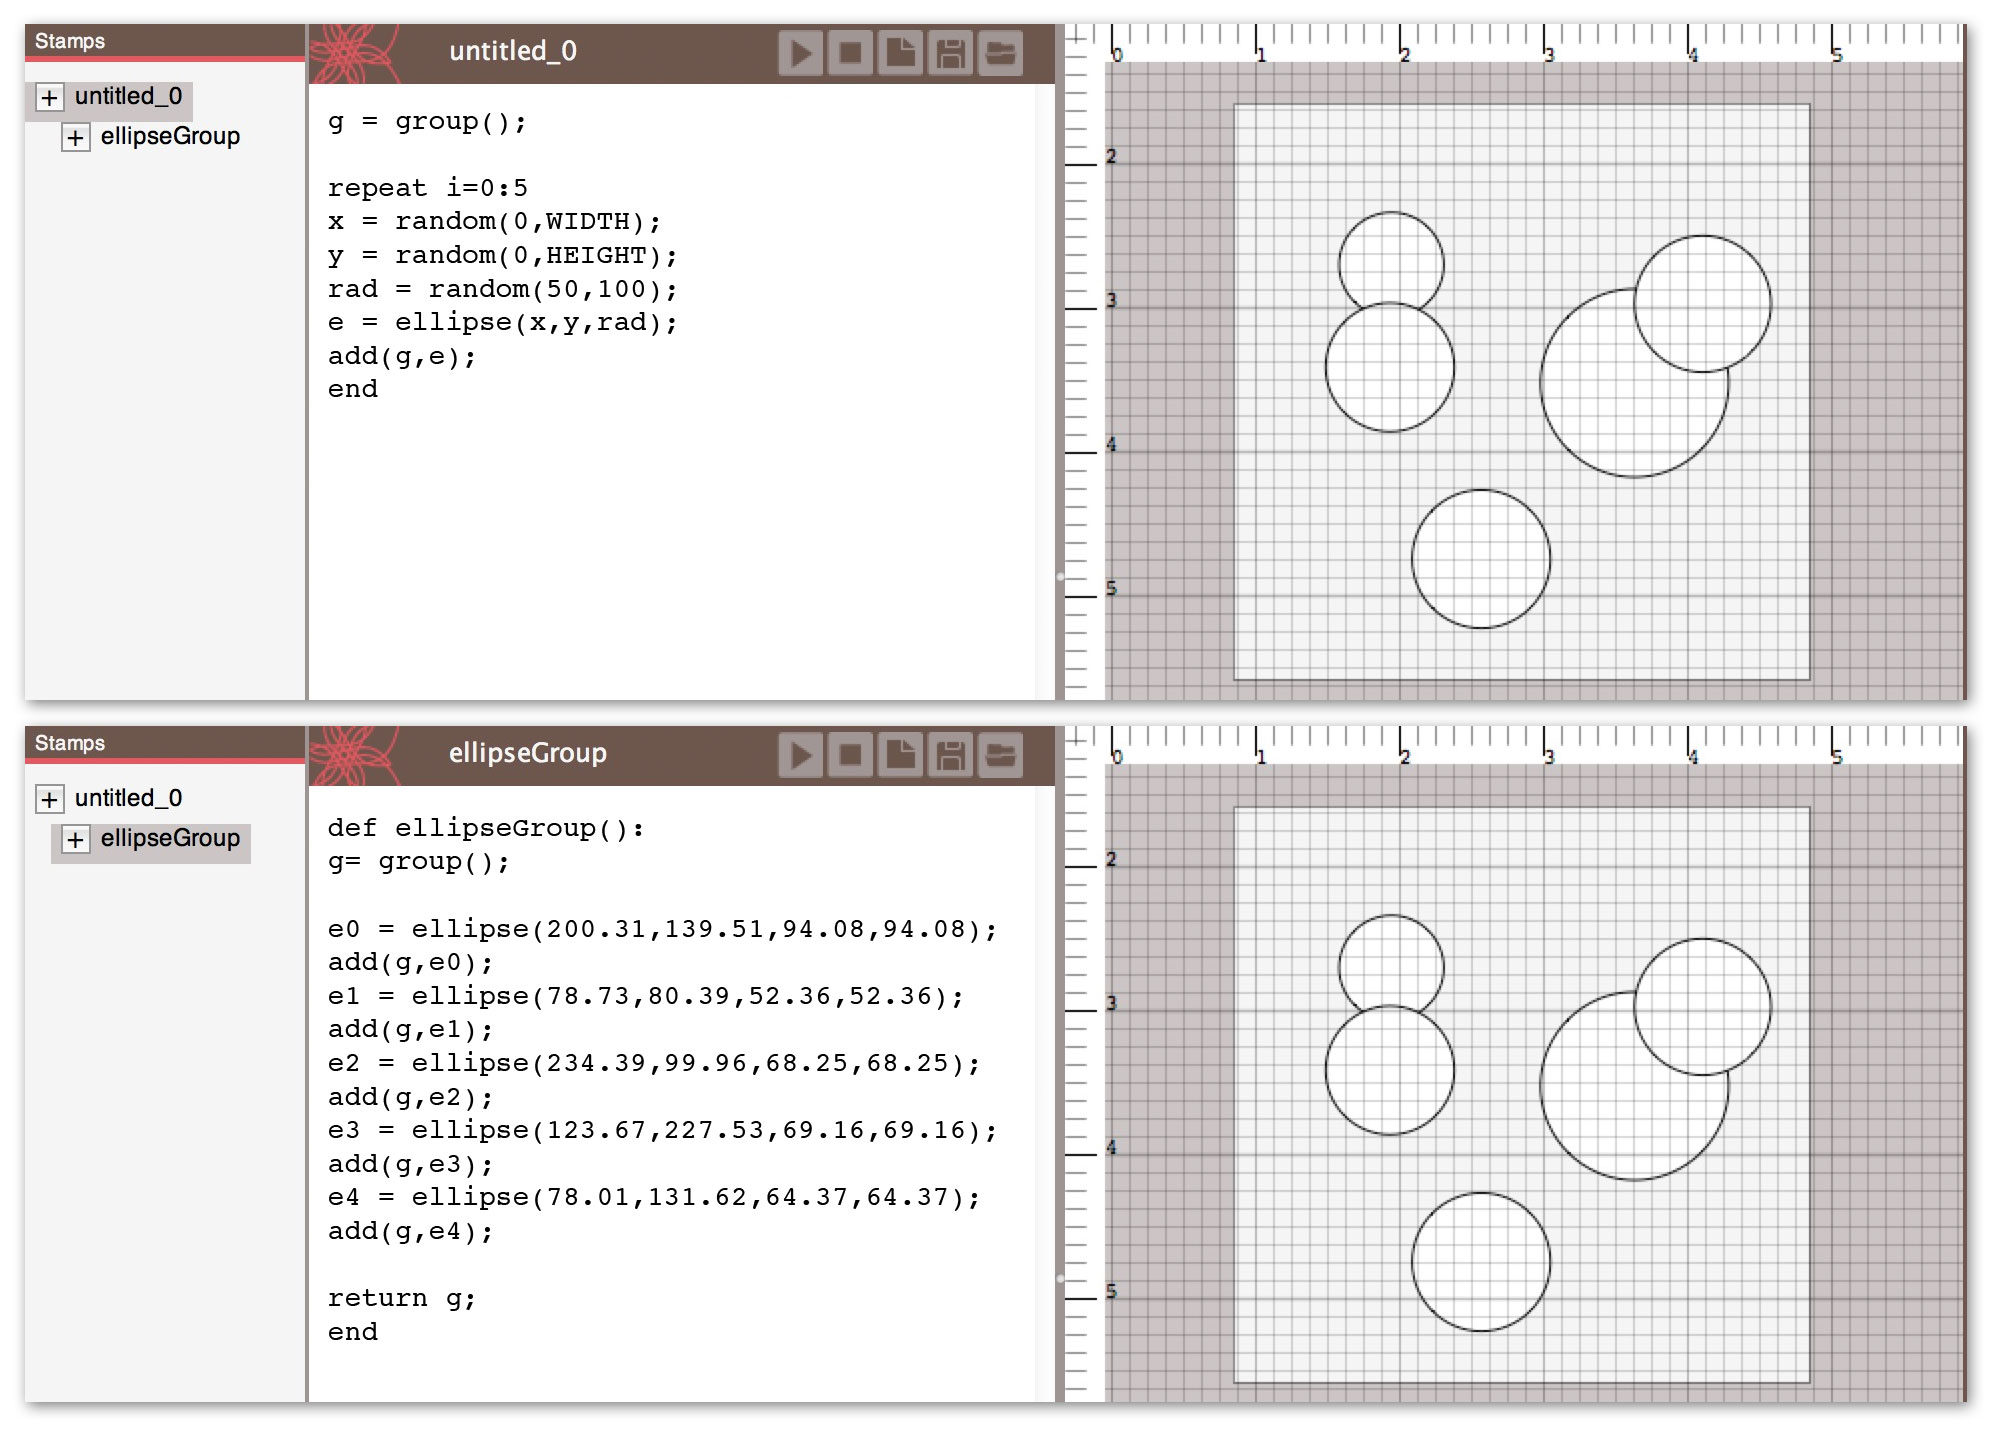
\includegraphics[width=\columnwidth]{images/stamps.jpg}
\caption{Static stamp functionality. (Top: User defined code which generates five random ellipses. The ellipses' positioning and size will change each time the program is run. Bottom: static stamp created from ellipses which will always return the same design.)}
\label{fig:stamps}
\end{figure}
\end{center}
\vspace{-20pt}

\subsection{Readability}
As we discovered through our implementation, Symmetry between graphic manipulation and textual programing must be tempered by concerns of usability. Merely producing a textual expression that accurately reflects a graphic action does not ensure that the interaction will be interpretable to the designer, let alone useful to their design process. We therefore attempted to make the editable linkages between programmatic and graphic actions to our target designs: novice programmers. 

\subsubsection{Expression Insertion}
First, we considered \textit{where} generated expressions appear within a program. For graphic action that initialize a new shape, the programming expression will always appear below the last line in the program. If the designer performs a transformation graphic action however, the expression will be inserted into the line below the last transformation expression of the selected shape, thereby automatically grouping shape initialization expressions with their corresponding transformations. Some of the transformation methods, including shape booleans and grouping methods result in the initialization of new shapes by combining several existing shapes. Any transformation expressions for these new shapes will subsequently appear following their initialization expression.  This results in the creation of a logically organized program through graphic edits.Naturally, in the process of manually writing code, the designer may consciously or unconsciously write expressions in a manner that deviates from this organization. Fortunately, manual edits by the designer will not prevent the auto generation method from functioning for successive graphic actions. More importantly, the consistent, simple rule-set for auto-insertion enables the designer to anticipate where expressions will be inserted into their code, which is essential as a program grows in length and complexity.

\subsubsection{Reference}
We also considered \textit{how} shapes should be referenced when transitioning between graphics and code. Similar to many functional programing languages, the DressCode language enables methods to be nested within one-another. Furthermore, there is no \textit{draw} method. Shapes that are initialized automatically appear in a design. Therefore there is a degree of flexibility and ambiguity for how a designer may employs identifiers in their code. In order to deal with this ambiguity when translating graphic actions to programmatic representations, we considered what would make a program most readable for a design. All graphic actions that create new shapes produce programmatic expressions that are automatically assigned an identifier. Subsequent transformation graphic actions will produce programmatic expressions that reference auto generated identifier on the following line. This produces code that while requiring more lines, is readable. In the case that the design problematically initializes a shape without an identifier and then transforms it graphically, the software will recognize the distinction and resort to wrapping the initialization expression in the appropriate transformation expression. if the design re-assigns or modifies the identifier of a shape through a programmatic action, future graphic actions on the shape will recognize this modification and use the new identifier.     

\subsubsection{Imperative History}
It was important to us that the steps used to arrive at a design were also readable. Because the DressCode programing language employs an imperative paradigm, designs are represented as a series of the designer's actions, rather than a single state which is updated as changes are made. We developed the linkages between graphic actions so that the programatic expressions also reflected the steps a designer made in the graphic interface. DressCode takes a verbose approach to generating programming expressions. For example, when a shape is moved with the move tool, a textual move expresssion is inserted into the designer's program. For all subsequent moves following the first move, rather than generate a successive string of additional move statements, the move expression is updated to reflect the new coordinates of the shape. However, if another tool is used to alter the shape, or a programatic expression is manually inserted by the designer to manipulate the shape, following the move statement, future actions with the move tool on the same shape will generate a new move statement, which will be subsequently updated until another tool is used (see Figure \ref{fig:auto_generated_code}).  This same logic applies to all other transformation tools in DressCode. We chose this structure, because it allows the program to preserve the designer's actions in the graphic panel as a series of discrete steps, thereby prodividng an opportunity  for the program to also serve as a means of reflection and evaluation on one's practice and design intentions. 

\subsection{Declarative Representations}
Although DressCode relies on an imperative paradigm, we recognized that a state-based representation could provide a useful means of illuminating the connections between the visual design and the textual program. Specifically, it was important to help a designer determine what code in their program was affecting specific shape in their design. Contemporary programing environments now frequently employ debug tools that allow the user to step through their code in an effort to dechipher its effects \cite{need citation}. Similarly many code editors contain declarative listings of all of the methods and identifiers in a class, providing an alternatve means of navigating one's code. We combined these tools in a way that is specific to a tool for programing and graphic drawing. DressCode features a declarative view which contains a listing of all primitives in the current design. Child primitives are nested within their parent groups. When selected in the declarative view, the primitive is selected and highlighted in the design view, and the line where the primitive was last modified in the text-editor is highlighted (see Figure \ref{fig:declarative_view}). The declarative view is designed to provide visual feedback on how elements of a design connect to the design's program, and provide a practical selection technique for complex designs.

\begin{center}
\begin{figure}[h!]
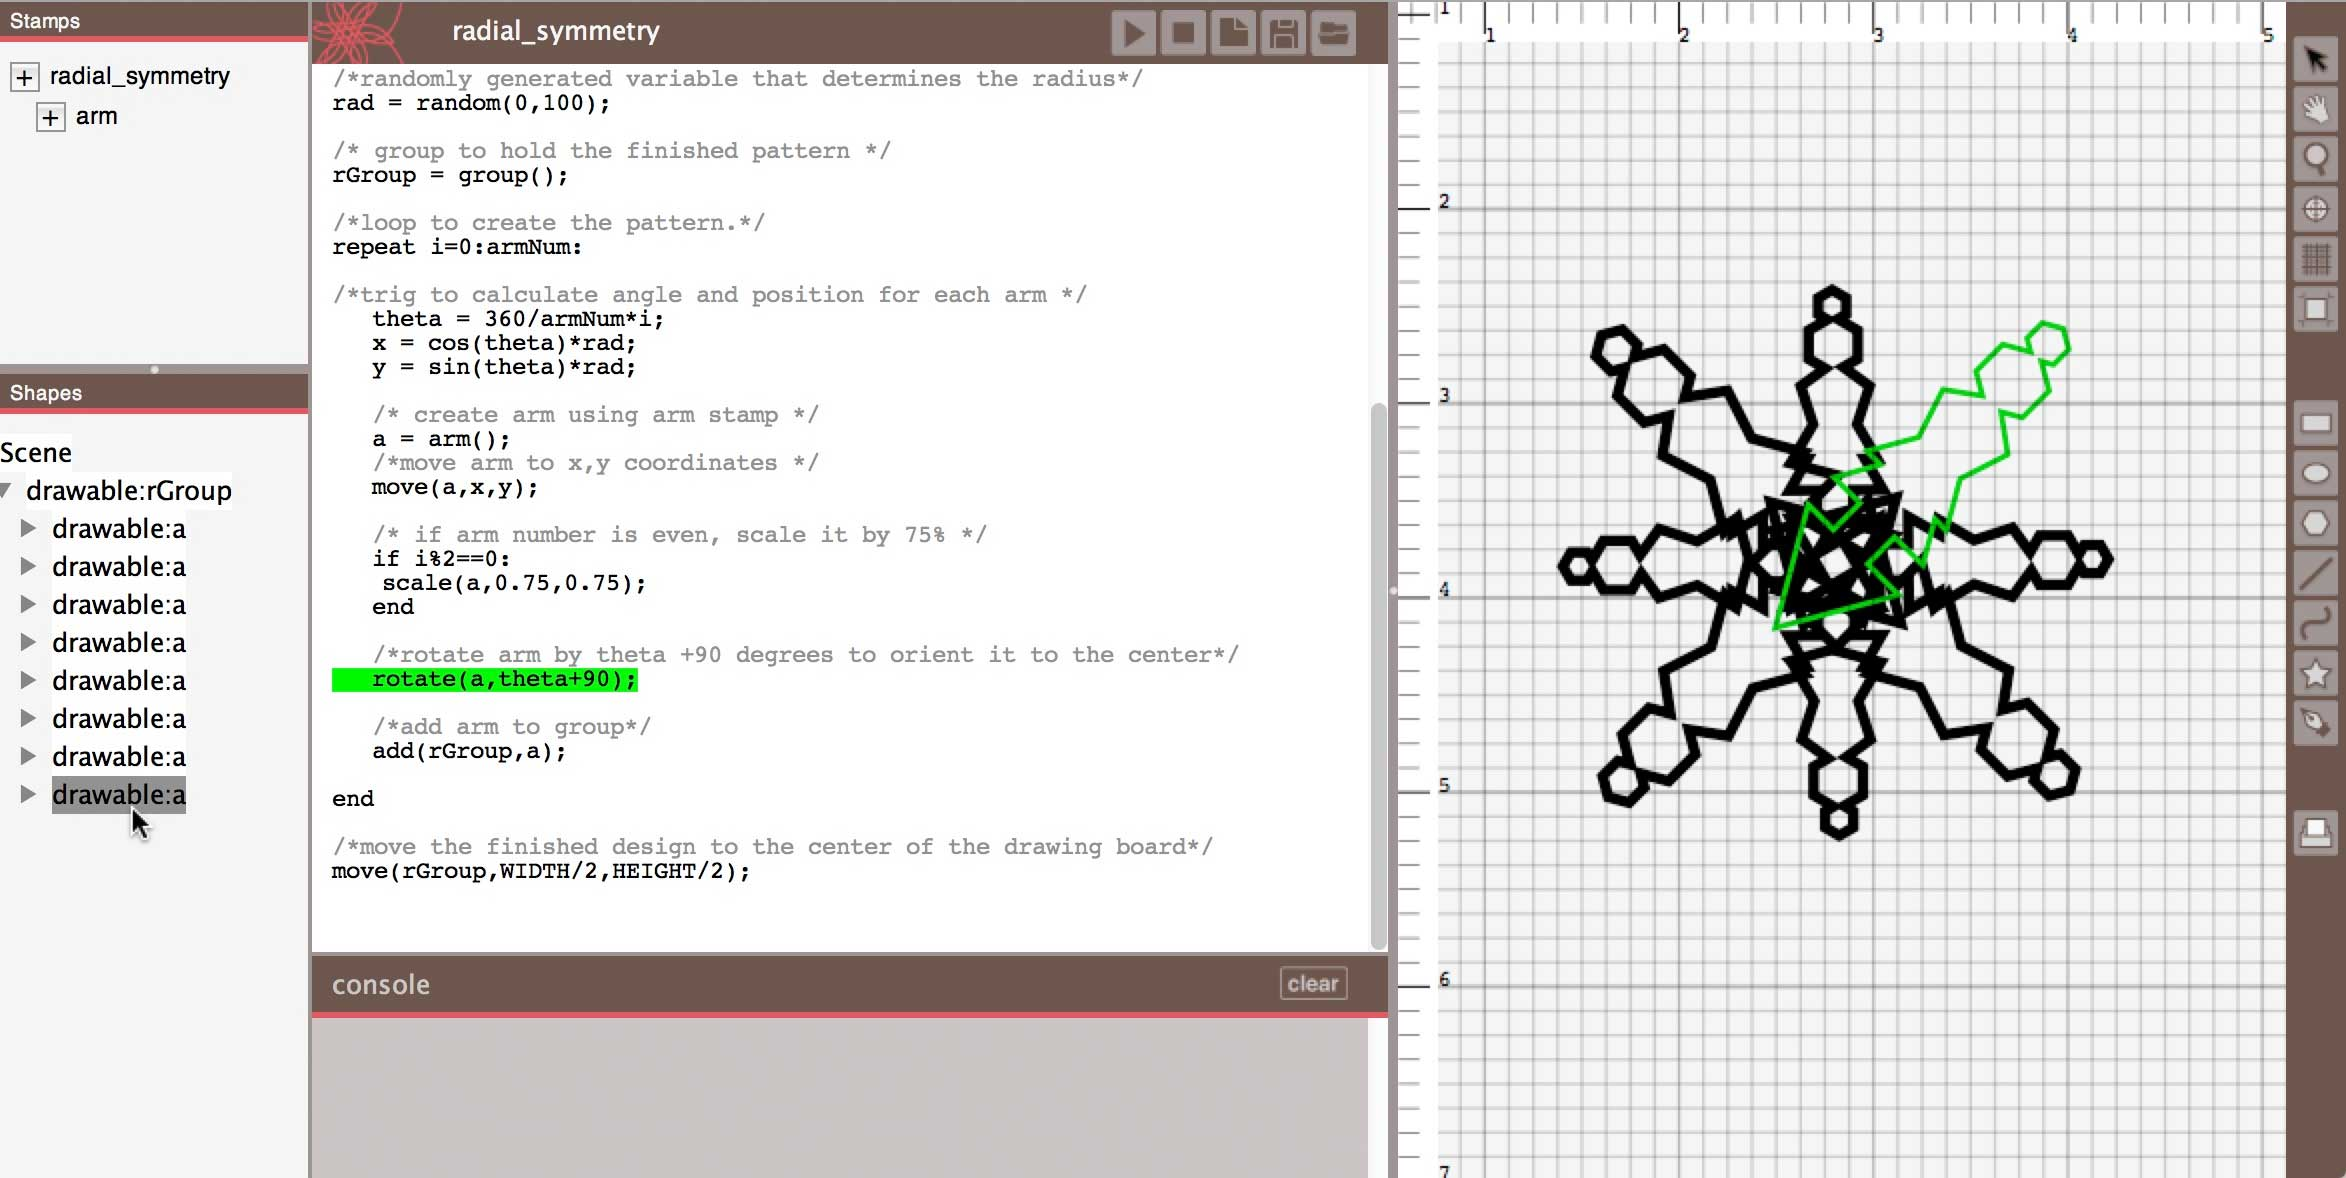
\includegraphics[width=\columnwidth]{images/selection_mechanism.jpg}
\caption{Declarative view with selected primitive}
\label{fig:declarative_view}
\end{figure}
\end{center}
\vspace{-20pt}

\subsection{Technical Implementation}
DressCode was developed as a Java-based application. The DressCode programming language is interpreted with semantic functionality that is simulated through a Java-based library. For most programs, interpretation is instantaneous; however, complex operations require several seconds to be executed. Here I can go into detail about how I built it, but maybe this is not important. If it is, I will write it later on. 

\section{Design Process}
 Technology use in the real world can be understood from an ecological perspective, where people's activities and tools adjust and are adjusted to each other in a complex system of interactions between norms, technical functionality and cultural values \cite{information_ecologies}. We developed DressCode with the objective of better understanding how a computational design tool could be effectively situated within the everyday lives of young people. In addition, we wished to incorporate a specific set values into our tool design which are frequently absent from mainstream technological use. It was necessary therefore that our design process and evaluation methods allowed us to understand the context in which our tool might be applied in the real world, and what values were reflected by this use. Our design process was to develop DressCode in an iterative fashion by testing successive versions in workshops with young people where they used the tool in the context of hand-craft applications to produce a finished artifact for their personal use. Here we elaborate on the values and specific evaluation behind DressCode, demonstrate the rationale for applying DressCode to craft, and describe our workshop methodology.

\subsection{Values and Evaluation Criteria}
By evaluating prior research in youth engagement in computational tools \cite{computational_thinking}, \cite{introductory_programing}, in conjunction to our own research motivations described in the introduction, we outlined set of value categories for DressCode, and corresponding evaluation critera.

\subsubsection{Accessibility}
 Although perhaps obvious when developing tools for novice use, accessibility is of paramount importance. To evaluate the accessibility of DressCode, we were concerned with the following questions: Could young programmers use the tool with a high degree of independence? What forms of experimentation and exploration were demonstrated? Were components of the tool intuitive to use? What level of confidence did people express in their use of the tool?

\subsubsection{Diversity}
 Whether performed by experts or novices, individual approaches to design are incredibly subjective and diverse \cite{learning_in_design}. It is essential then that computational design tools afford a diversity of practices. Drawing from Brennan and Resnick, we wish to value diverse forms of computational practice. Are participants able to meaningfully apply computational constructs to their design objectives? Are they able to remix other people's designs? Are they able to critique other's designs and offer technical and aesthetic advice \cite{computational_thinkng}? Does use of the tool produce a wide variety of end products? Beyond a diversity of design practices, what forms of diversity are exhibited by the people who are interested in using the tool? %this last sentence could be much better

\subsubsection{Relevancy}
  Despite our belief that computation can serve as a valuable tool for personal expression, people who are new to computer science often view computer programing as irrelevant to their personal interests \cite{introductory_programming}. It is important that our approach with DressCode allows for a reconciliation between computational practices and the values and goals of young people. We wonder how  artifacts created with DressCode may be used in daily lives of the people who made them. How long are they kept and cared for by their makers? Further, how might the use of DressCode alter perspectives towards the creative applications of programing?

\subsubsection{Engagement}
Note: Improve this section. Csikszentmihalyi’s research has demonstrated the importance of personal motivation and enjoyment in high levels of achievement, particularly in the case of young people \cite{csiks}.  In developing our tool, we were concerned with specific behaviors that we believe could be used as indicators of a deep engagement in the creative application of computational tools. Do users of the tool demonstrate motivation to take on difficult tasks? Do participants take pride in their artifacts and exhibit care and attention to detail in their creation? Do people express an interest in future participation in similar activities? 

\subsubsection{Social Connections}
A common perspective of computer programing is that it is an asocial and solitary activity \cite{introductory_programing}. Because we recognize that social engagement is a core component of a young person's life, as well as a necessary element of creativity, we seek to promote forms of computational engagement that emphasize social connections, and evaluate DressCode by how it enables people to work together. In particular, we wish to foster forms of creation where the process of creating with others is a central component of an activity, leading to forms of social interaction with peers which are both pleasurable and productive. 

\subsection{Craft Application}
Craft based approaches offer powerful way to engage young people in computation, and in particular offer the opportunity to reach under-respresented demographics like young women. Most frequently, craft has been connected to electronics and physical computing enabling the integration of electronic actuation, sensing and interactivity into craft artifacts \cite{dave}, \cite{kit_of_no_parts}, \cite{jie}, \cite{leah_lilypad}. These combinations have been effective in enaging novice programers and non-traditional user groups. Inspired by this work, we chose to combine craft and computing in a different way, by developing tools to enable the computational design of the visual and physical forms of craft artifacts. We anticipated that this approach would allow for many of the rich properties of craft to be combined with the unique design principles of computational design. The properties of craft we are interested in are as follows:
MAKE THESE SPECIFIC TO HOW THEY EXTEND COMPUTATIONAL DESIGN and factor into our original objectives (relevancy, accessibility, diversity, engagement)
\subsection{Properties of Craft}
\begin{itemize}
\item \textbf{Materiality:} Craft involves working with physical materials by hand. Intuitive decisions are made while physically manipulating the material. 
\vspace{-6pt}
\item \textbf{Pleasure through physical labor:} Fundamental to traditional conceptions of arts and crafts is the idea of pleasure in working with one's hands \cite{abstracting_craft}.
\vspace{-6pt}
\item \textbf{Unification of form and function:} Many forms of craft can applied the creation of objects that merge ornamental and useful qualities.
\vspace{-6pt}
\item \textbf{Craftsmanship:} Traditional notions of craft are closely connected to the idea craftsmanship: the motivation to produce quality work for its own sake \cite{the_craftsman}.
\end{itemize}


\section{Workshops}
\subsection{Workshop 1}
\subsection{Workshop 1 Results}
\subsection{Design Revisions}
\subsection{Workshop 2}
\subsection{Workshop 2 Results}

\section{Discussion}
\subsection{Accessibility}
\subsection{Diversity}
\subsection{Relevancy}
\subsection{Engagement}
\subsection{Social Connections}

\section{Conclusion}

% REFERENCES FORMAT
% References must be the same font size as other body text.

\bibliographystyle{acm-sigchi}
\bibliography{dresscode}
\end{document}